\graphicspath{{03-Ckov/Figures/}}

\section{Cherenkov Detectors}
\label{Sect:Ckov}

\subsection{Introduction}
\label{SubSect:Ckov_Intro}
% Lucien Cremaldi (and David Sander) reviewed this

The MICE Cherenkov threshold detectors, measuring velocity, are primarily designed to provide $\pi$-$\mu$ separation in the higher momentum ranges, where TOF peaks separation is not sufficient for conclusive particle identification.

In order to provide separation over a large range of momenta, two high density silica aerogel Cherenkov detectors (CkovA and CkovB) with refractive indices $n$=1.07 and $n$=1.12 are used.
Light is collected in each counter by four 9354KB eight-inch UV-enhanced phototubes and recorded by CAEN V1731 FADCs (500~MS/s).
The two detectors are placed directly one after another in the beamline, located just after the first TOF counter. In~Fig.~\ref{fig:ckov1} an exploded view of one detector is shown.

Their respective thresholds provide different responses in four distinct momentum ranges, i.e. in the 200 MeV/$c$ beams, pions are below the threshold which would fire the detector for both CkovA and CkovB whereas muons are above only for CkovB, while for the 240 MeV/$c$ beams, pions are above the threshold for CkovB while muons are above for both CkovA and CkovB. Using this information algorithms can be written that produce likelihood distributions of particle type.
Below the CkovB muon threshold of about 217.9~MeV/$c$, where there is no separation, the TOFs provide good separation, whereas the momentum range above the CkovA pion threshold 367.9~MeV/$c$ is outside of the MICE running parameters~\cite{NOTE473}.
For unambiguous identification of particle species the Cherenkov detectors would need a momentum measurement from the MICE Tracker.

\begin{figure}[htb!]
  \begin{center}
    \includegraphics[width=0.6\columnwidth]{./03-Ckov/Figures/Ckov.png}
    \caption{MICE aerogel Cherenkov counter blowup: a)~entrance window, b)~mirror, c)~aerogel mosaic, d)~acetate window, e)~GORE reflector panel, f)~exit window and g)~eight-inch PMT in iron shield.}
    \label{fig:ckov1}
  \end{center}
\end{figure}

\subsection{Performance}
\label{SubSect:Ckov_Performance}

The data sets used to evaluate the Cherenkov detectors are summarized in Table~\ref{tab:ckov}. A wide range of settings (including alignment runs) has been used in order to cover the full spectra of particles that could have been measured by the detectors.

\begin{table}
  \begin{center}
    \begin{tabular}{c|c|c|c|c}
       Run ID & Date & Nominal momentum [MeV/$c$] & Spills & Triggers \\
  		\hline
       10488  & 12/12/2017 & 140 & 3777 & 300269 \\
       10496  & 12/12/2017 & 170 & 4180 & 371037 \\
       10391  & 03/12/2017 & 200 & 2146 & 240033 \\
       10419  & 04/12/2017 & 240 & 2932 & 328062 \\
       10304  & 29/11/2017 & 300 & 2502 & 305363 \\
       10221  & 23/11/2016 & 300 & 4493 & 560119 \\
       10519  & 15/12/2017 & 400 & 4316 & 506384 \\
    \end{tabular}
   \caption{Summary of the data sets used to visualize the activation curve of the MICE Cherenkov detectors.}
   \label{tab:ckov}
  \end{center}
\end{table}

The asymptotic light yield (for $\beta$=$v$/$c$=$1$) in each counter has been measured using the electron peaks, giving $16\pm1$ photoelectrons (NPE) in CkovA and $19\pm1$ in CkovB.

The photoelectrons yields versus momentum for muons and pions in CkovA and CkovB are displayed in Fig.~\ref{fig:ckov2}, using the time of flight between TOF0 and TOF1 to select the species and estimate the momenta.
The distributions of NPEs as a function of the momentum P have been fitted with the function

\begin{equation}
NPE(P) = NPE_0 + NPE_{\beta=1}\left(1-\left(\frac{P_0}{P}\right)^2\right)
\end{equation}

where $NPE_0$ is the number of background photoelectrons, $NPE_{\beta=1}$ is the asymptotic light yield and $P_0$ is the momentum threshold.

\begin{figure}[htb!]
  \begin{center}
    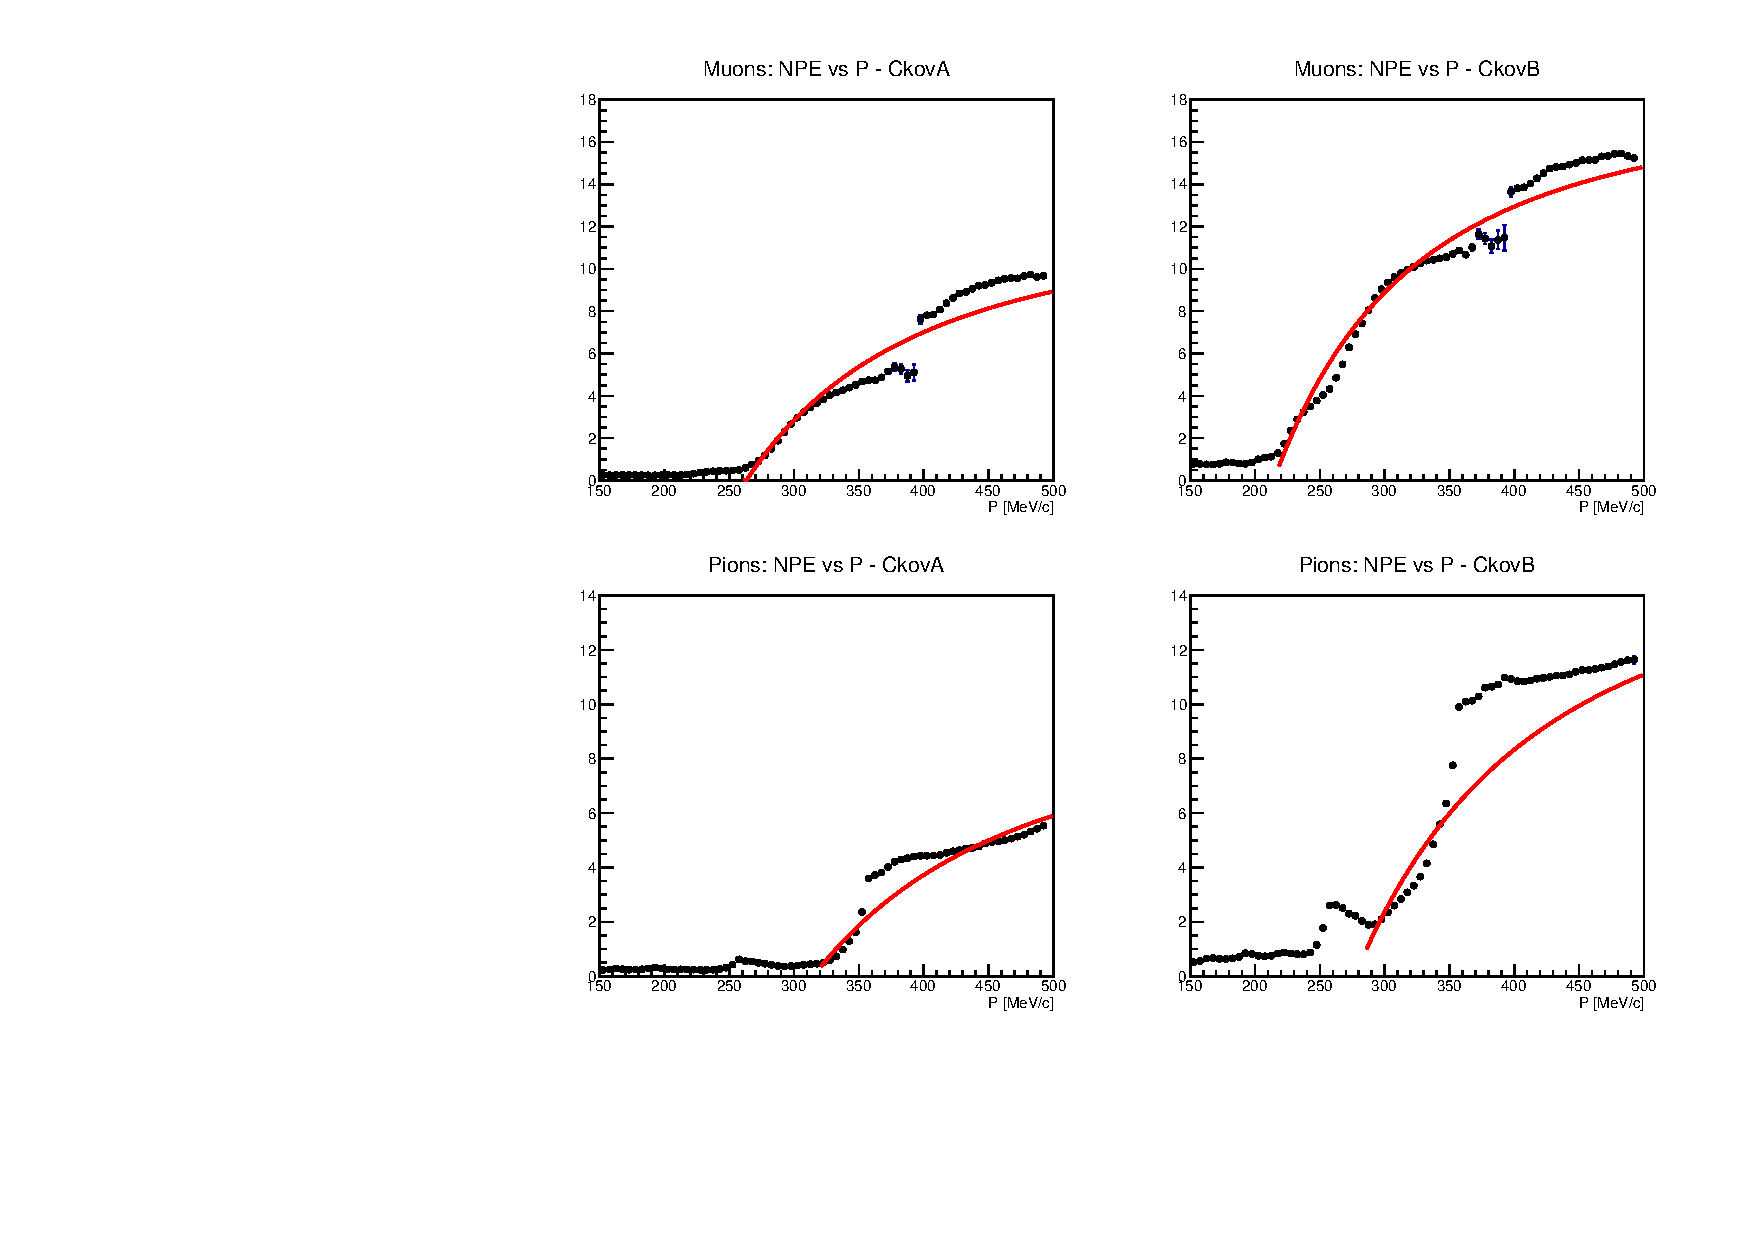
\includegraphics[width=0.85\columnwidth]{./03-Ckov/Figures/Ckov_photoelectrons_vs_P.pdf}
    \caption{Photoelectron yields versus momentum for muons and pions in CkovA and CkovB with the superimposed fitted activation functions.}
    \label{fig:ckov2}
  \end{center}
\end{figure}

The observed muon thresholds are $267.2\pm5.2$ and $220.0\pm16.9$ MeV/$c$, while for pions are $331.8\pm16.4$ MeV/$c$ and $296.1\pm0.1$ MeV/$c$, respectively in CkovA and CkovB. The $NPE_{\beta=1}$ values are generally lower than the values predicted as in a previous analysis~\cite{NOTE473} done with Step~I data: this is mostly due to TOF0 acting as a pre-shower radiator.

In Fig.~\ref{fig:ckov3} is shown the typical photoelectron spectra for muons and pions well above the threshold. The expected Poisson-like distribution got tails from the electromagnetic showers and from secondary electrons coming from interactions in TOF0 and in the aerogel itself.

\begin{figure}[htb!]
  \begin{center}
    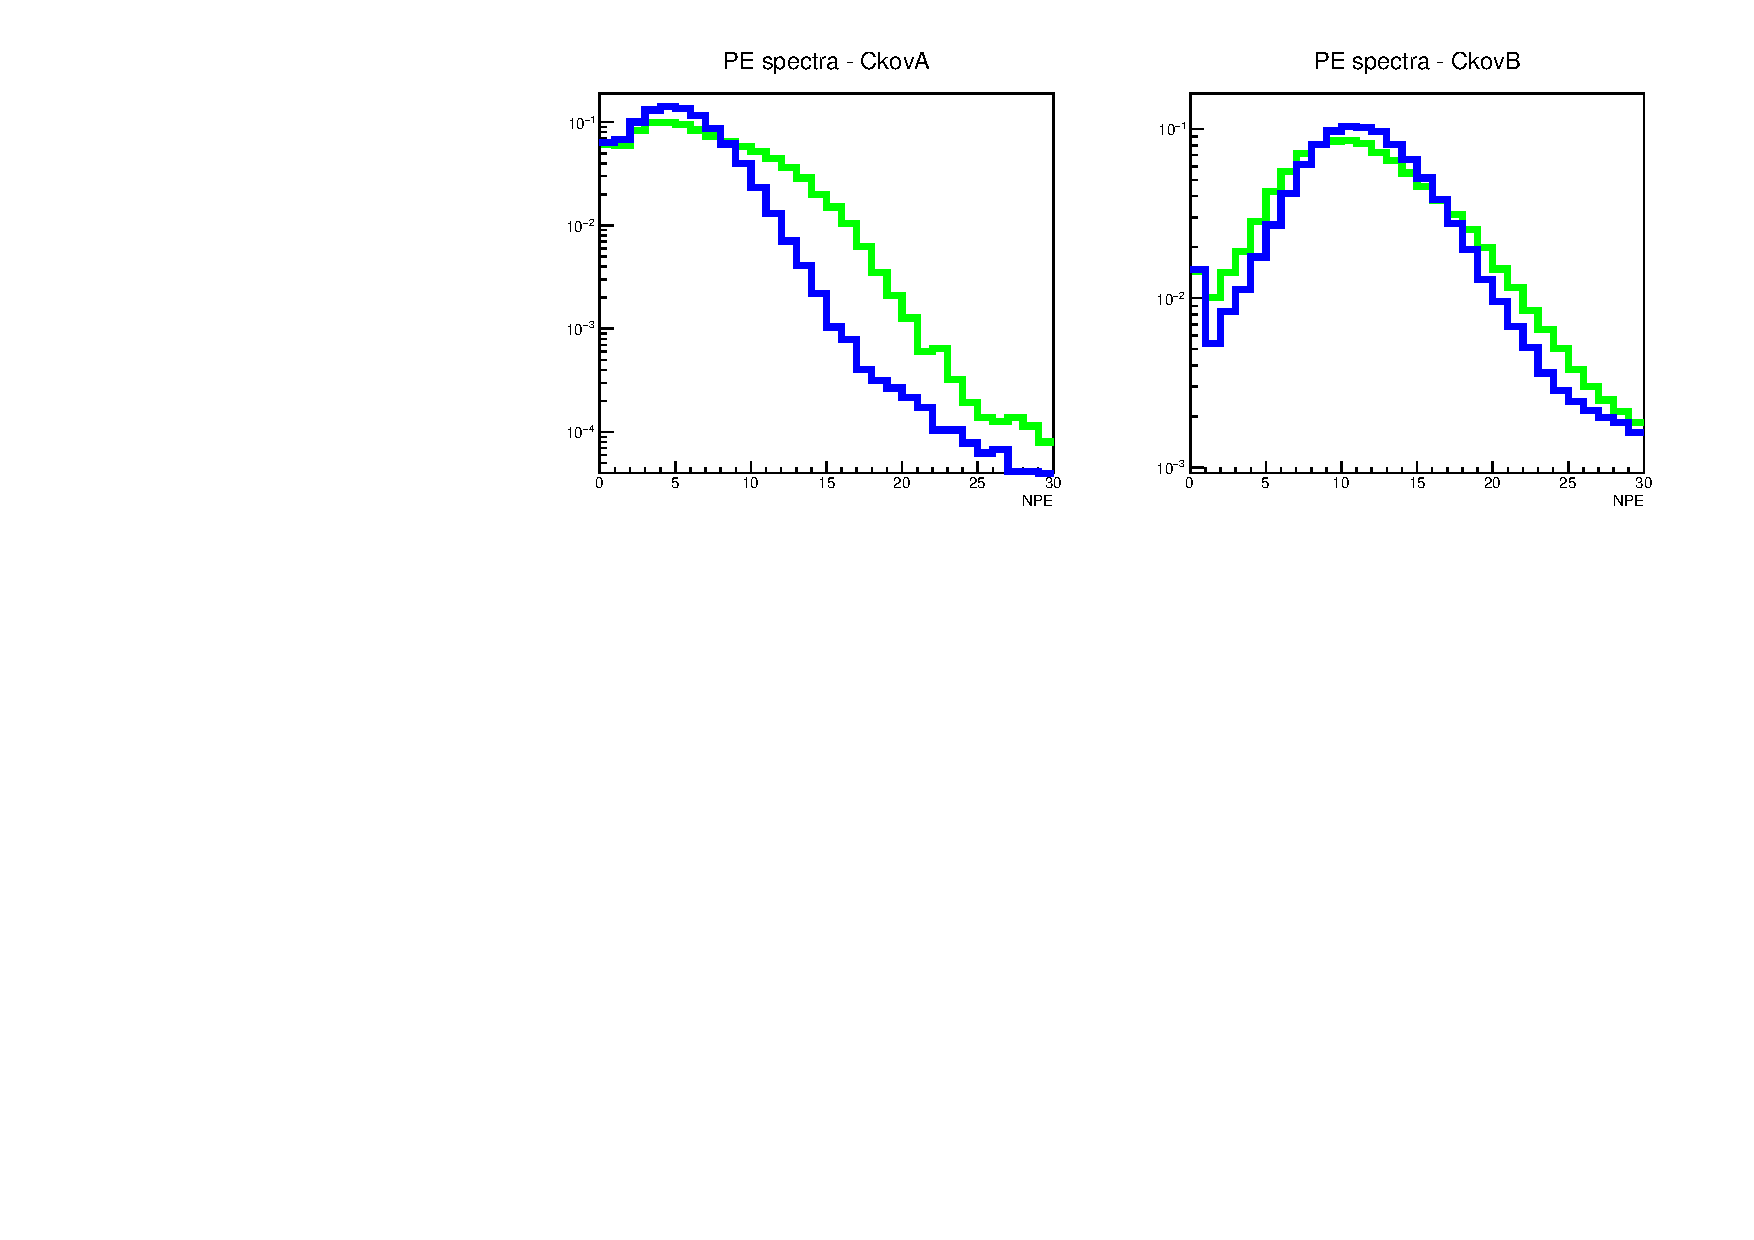
\includegraphics[width=0.85\columnwidth]{./03-Ckov/Figures/Ckov_photoelectrons_spectra.pdf}
    \caption{Photoelectron spectra in CkovA (left) and CkovB (right) for muons (green) and pions (blue) above the threshold. The distributions are both normalised.}
    \label{fig:ckov3}
  \end{center}
\end{figure}
